


\section{Tratamento dos dados}

\textbf{Normalização} \par
A normalização foi deixada por ser aprendida nos modelos, sendo que todos têm como segunda camada, uma de normalização.\par

\textbf{Limpeza} \par

Podemos ver pelos gráficos seguintes que a existem alguns outliers, sendo estes definidos como 3 desvios padrão de distância à média.\par
Estes gráficos mostram também que existe uma variação do que são os valores normais de cada atributo a nível temporal. Logo um método de limpeza não se poderia basear apenas numa definição geral de outliers, mas teria de ser feito em janelas temporais.\par
Pelo mesmo argumento e visto que os outliers fazem parte do que queremos também descobrir, não é aplicada nenhum método de remoção dos mesmo, sendo os dados passados a cru para os modelos.\par


\begin{figure}[H]
  \centering
  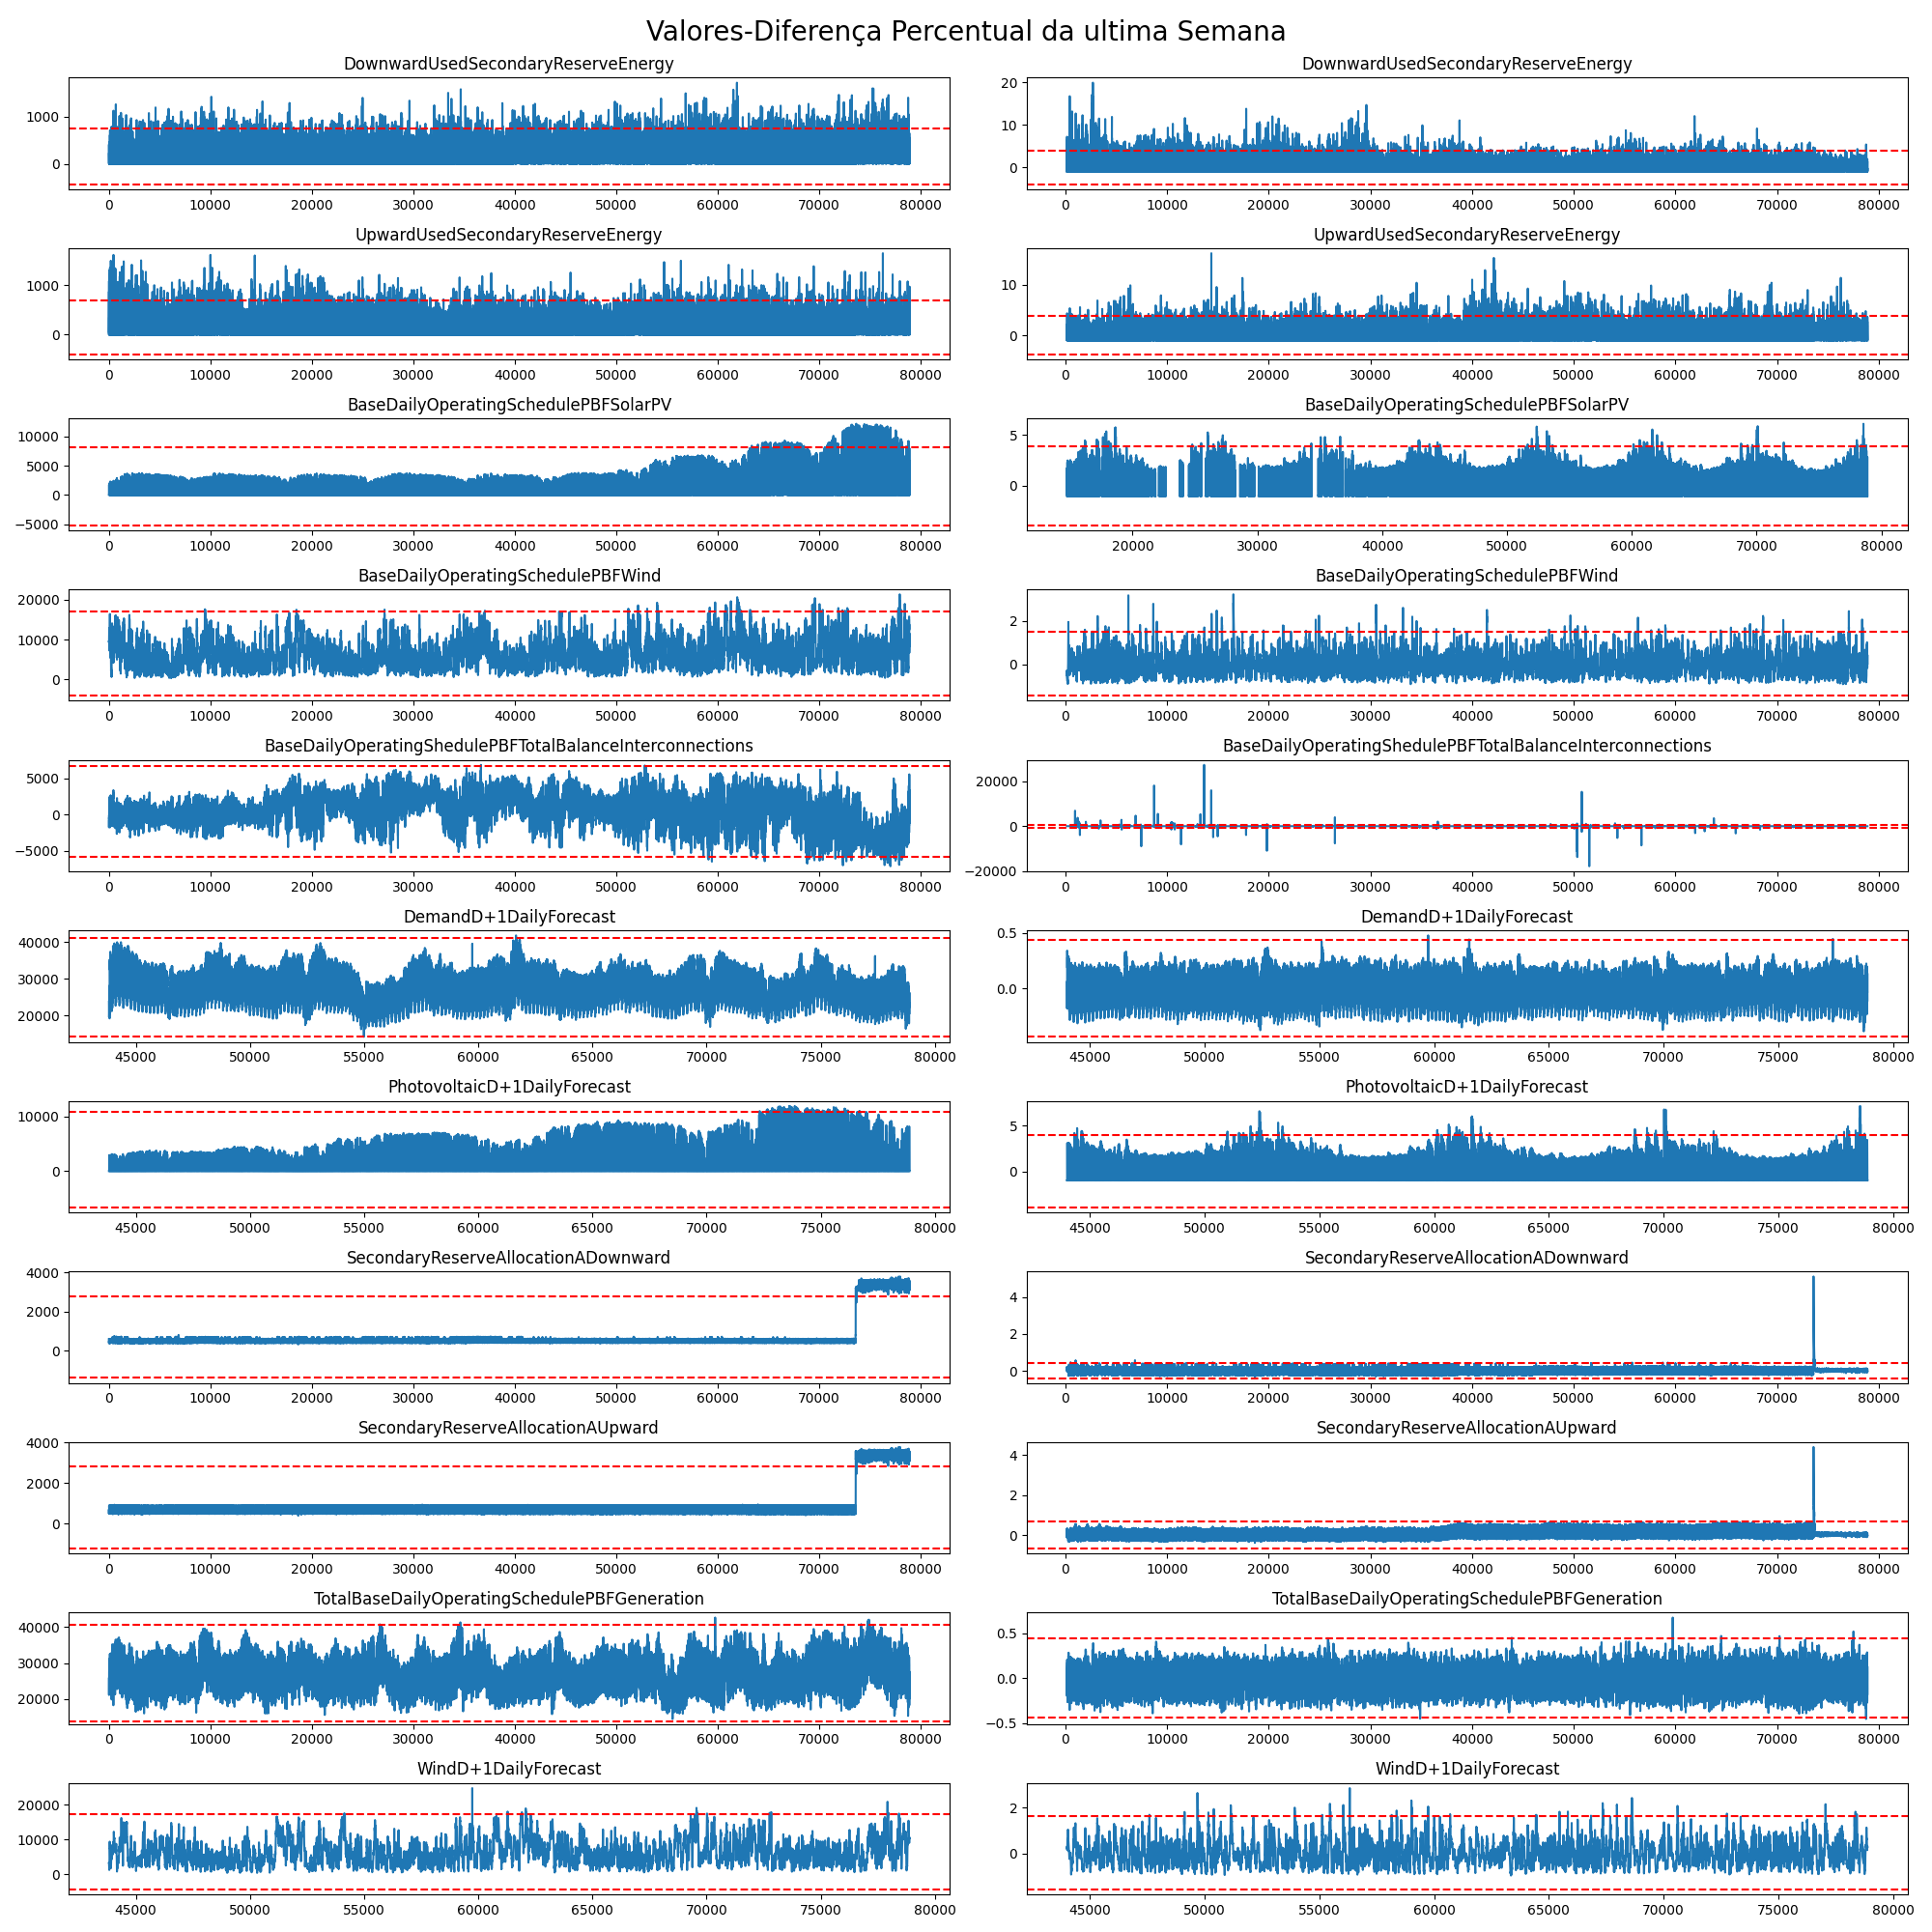
\includegraphics[width=\textwidth]{plots/Outliers_3stds.png}
  \caption{Outliers}
\end{figure}

Outra análise desta variação dos atributos a nível temporal leva-nos a que qualquer divisão dos dados para treino e teste deva levar as variações em consideração. Isto sendo que o treino deve ter representatividade de todas, ou maior parte, das condições diferentes.\par


\textbf{Dados em falta (Missing Data)}

Estudemos também o caso de dados em falta. Alguns destes atributos têm certas entradas vazias, e como podemos ver alguns não têm alguns anos inteiros.\par
Como queremos usar o máximo de dados possíveis iremos usar técnicas de imputing nesses dados.\par
Podemos ver que temos dados em falta de vários anos, em três atributos, e um tem algumas horas esporádicas em falta nos primeiros anos.\par

\begin{figure}[H]
  \centering
  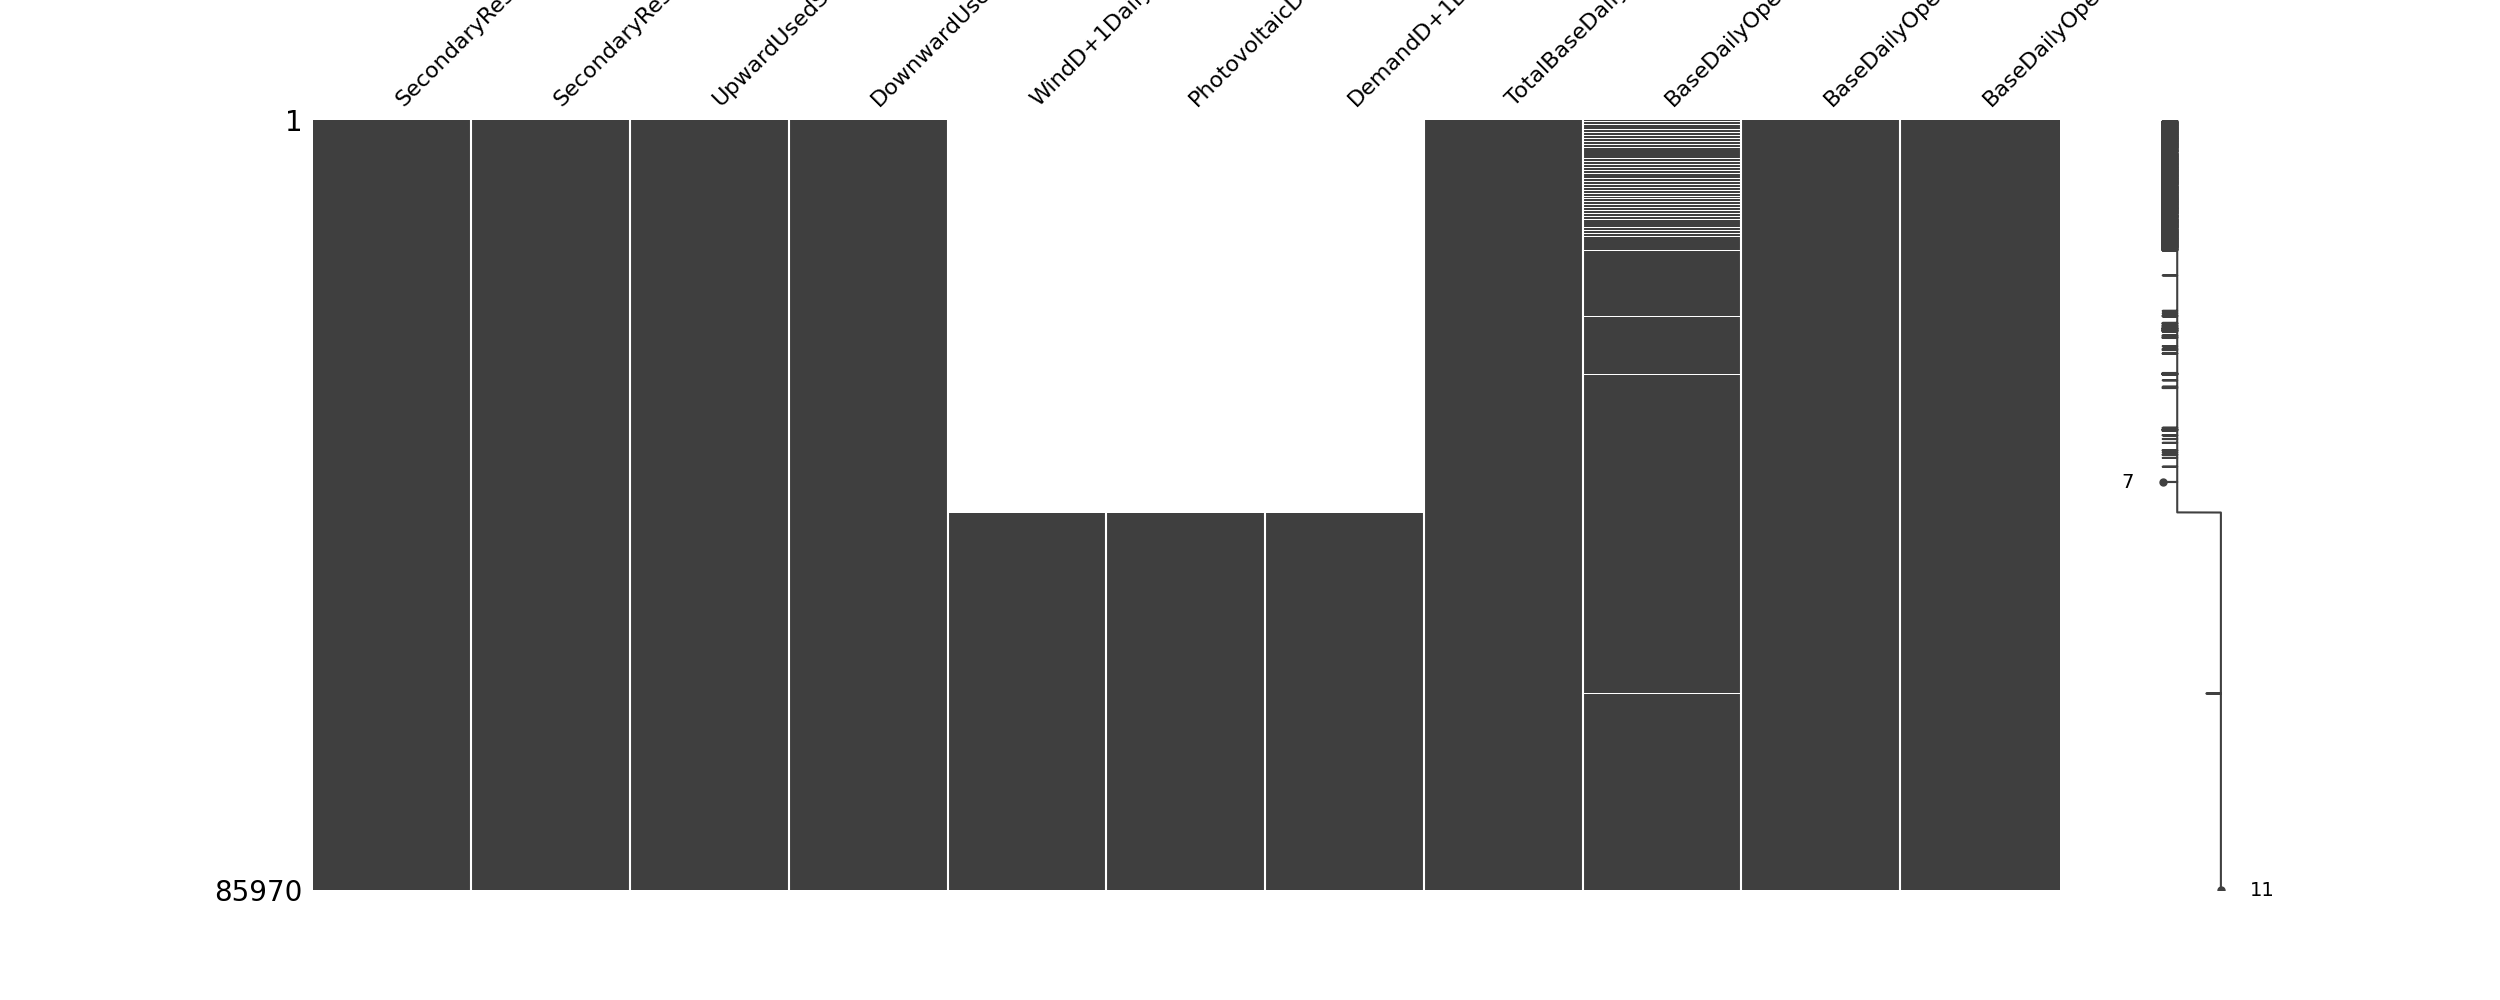
\includegraphics[width=\textwidth]{plots/missing_data.png}
  \caption{Dados em falta}
\end{figure}

Vamos aplicar o método experimental \href{https://scikit-learn.org/stable/modules/generated/sklearn.impute.IterativeImputer.html}{IterativeImputer} da biblioteca de python \href{https://scikit-learn.org/stable/index.html}{sklearn}.\par
Este metodo é baseado nos trabalhos de \cite{vanBuuren2011} e de \cite{Buck1960}.\par
Por ultimo foi adicionado ao dados mais atributos, sendo eles todos de cariz temporal. É adicionado atributos correspondentes à hora, ao dia do ano, ao dia da semana, ao dia do mês, mês, ano.\par

